\documentclass[11pt]{IEEEtran}
\usepackage{graphicx}
\begin{document}

\title{Enterprise Database Products}


\author{Amarjeet Singh Kapoor, 1311015, D3 CSE A1, amarjeet.kapoor1@gmail.com}



% The paper headers




% make the title area
\maketitle


\begin{abstract}
Relational Database Management Systems have become a very rigorous
part of a general person's life from a service point of view.And they
are of even paramount importance for a computer science student/
practitioner from a applicability point of view.There is considerable interest in studying DBMS applications from a
computer science engineer's perspective.  It is a historical field but
one with great future scope as well.Newer and newer advancements are
being made in order to provide efficient, effective and cost friendly
data solution to various industries and enterprises.To fulfil both these roles many software RDBMS products are available
in the market presently. But only a few of them enjoy popularity and
acceptance from the developer and industrial community. This report/
assignment is fundamentally concerned with studying a few epitomes of
Relational Database Management Systems. These include IBM DB2, Oracle,
Microsoft SQL server and MySQL.The primary purpose of this study is to present each of the above
mentioned software separately and illustrate their key features and
capabilities.  While there is some rich variety amongst these software
but it is important to understand that at the base level they are
doing the basic job of a DBMS, so it becomes very important for us to
study in detail how these software are actually different.

\end{abstract}



\section{IBM DB2}
IBM DB2 is a family of database server products developed by IBM. These products all support the relational model, but in recent years some products have been extended to support object-relational features and non-relational structures like JSON and XML.
\subsection{History}
DB2 traces its roots back to the beginning of the 1970s when Edgar F. Codd, a researcher working for IBM, described the theory of relational databases and in June 1970 published the model for data manipulation.

In 1974 the IBM San Jose Research center developed a relational DBMS, System R, to implement Codd's concepts.�A key development of the System R project was SQL. To apply the relational model Codd needed a relational database language he named DSL/Alpha. At the time IBM didn't believe in the potential of Codd's ideas, leaving the implementation to a group of programmers not under Codd's supervision, who violated several fundamentals of Codd's relational model; the result was Structured English QUEry Language or SEQUEL. When IBM released its first relational database product, they wanted to have a commercial-quality sublanguage as well, so it overhauled SEQUEL and renamed the basically new language Structured Query Language (SQL) to differentiate it from SEQUEL. The acronym SEQUEL was changed to SQL because ``SEQUEL" was a trademark of the UK-based Hawker Siddeley aircraft company.

IBM bought Metaphor Computer Systems to utilize their GUI interface and encapsulating SQL platform that had already been in use since the mid 80's. In parallel with the development of SQL IBM also developed Query by Example (QBE), the first graphical query language.

IBM's first commercial relational database product, SQL/DS, was released for the DOS/VSE and VM/CMS operating systems in 1981. In 1976 IBM released Query by Example for the VM platform where the table-oriented front-end produced a linear-syntax language that drove transactions to its relational database.Later the QMF feature of DB2 produced real SQL and brought the same ``QBE" look and feel to DB2.

The name DB2, or IBM Database 2, was first given to the Database Management System or DBMS in 1983 when IBM released DB2 on its MVS mainframe platform. 
\subsection{Editions}
IBM has changed the packaging structure in the latest release of DB2 for Linux, Unix and Windows and now offers seven editions: Advanced Enterprise Server Edition, Advanced Workgroup Server Edition, Enterprise Server Edition, Workgroup Server Edition, Express Edition, Developer Edition and Express-C. Each of these editions have been packaged for different deployment scenarios and workloads Applications built for lower editions of DB2 are guaranteed to work on higher editions but at a higher level of performance.
\subsection{Technical Information}
DB2 can be administered from either the command-line or a GUI. The command-line interface requires more knowledge of the product but can be more easily scripted and automated. The GUI is a multi-platform Java client that contains a variety of wizards suitable for novice users. DB2 supports both SQL and XQuery. DB2 has native implementation of XML data storage, where XML data is stored as XML (not as relational data or CLOB data) for faster access using XQuery.

DB2 has APIs for REXX, PL/I, COBO, RPG, FORTRAN,�C++, C, Delphi,�.NET CLI, Java, Python, Perl, PHP, Ruby and many other programming languages. DB2 also supports integration into the Eclipse and Visual Studio integrated development environments.
\subsection{Error Processing}
An important feature of DB2 computer programs is error handling. The SQL communications area (SQLCA) structure was once used exclusively within a DB2 program to return error information to the application program after every SQL statement was executed. The primary, but not singularly useful, error diagnostic is held in the field SQL CODE within the SQLCA block.
The SQL return code values are:-
\begin{itemize}
\item 0 means successful execution.
\item A positive number means successful execution with one or more warnings. An example is +100, which means no rows found.
\item A negative number means unsuccessful with an error. An example is -911, which means a lock timeout (or deadlock) has occurred, triggering a rollback.
\end{itemize}

Later versions of DB2 added functionality and complexity to the execution of SQL. Multiple errors or warnings could be returned by the execution of an SQL statement; it may, for example, have initiated a Database Triggerand other SQL statements. Instead of the original SQLCA, error information should now be retrieved by successive executions of a GET DIAGNOSTICS statement.
See SQL return codes for a more comprehensive list of common SQLCODEs.


\section{Oracle Database}

Oracle Database�(commonly referred to as Oracle RDBMS or simply as Oracle) is an object-relational database management system produced and marketed by Oracle Corporation.
\subsection{History}
Corporate/technical timeline:
\begin{itemize}

\item 1977: Larry Ellison and friends founded Software Development Laboratories (SDL).
\item 1978: Oracle Version 1, written in assembly language, runs on PDP-11 under RSX, in 128K of memory. Implementation separates Oracle code and user code. Oracle V1 is never officially released. 
\item 1979: SDL changed its company-name to "Relational Software, Inc." (RSI) and introduced its product Oracle V2 as an early relational database system - often cited as the first commercially sold RDBMS. The version did not support transactions, but implemented the basic SQL functionality of queries and joins. (RSI never released a version 1 - instead calling the first version version 2 as a marketing gimmick.) 
\item 1982: RSI in its turn changed its name, becoming known as "Oracle Corporation", to align itself more closely with its flagship product.
\item 1983: The company released Oracle version 3, which it had re-written using the C programming language, and which supported COMMIT and ROLLBACK functionality for transactions. Version 3 extended platform support from the existing Digital VAX/VMS systems to include Unix environments. 
\item 1984: Oracle Corporation released Oracle version 4, which supported read-consistency. In October it also released the first Oracle for th �IBM PC. 
\item 1985: Oracle Corporation released Oracle version 5, which supported the client/server model a sign of networks becoming more widely available in the mid-1980s.
\item 1986: Oracle version 5.1 started supporting distributed queries.
\item 1988: Oracle RDBMS version 6 came out with support for PL/SQL embedded within Oracle Forms v3 (version 6 could not store PL/SQL in the database proper), row-level, locking and hot backups. 
\item 1989: Oracle Corporation entered the application-products market and developed its ERP product, (later to become part of the Oracle E-Business Suite), based on the Oracle relational database.
\item 1990: the release of Oracle Applications release 8
\item 1992: Oracle version 7 appeared with support for referential integrity, stored procedures and triggers.
\item 1997: Oracle Corporation released version 8, which supported object-oriented development and multimedia applications.
\item 1999: The release of Oracle8i aimed to provide a database inter-operating better with the Internet (the i in the name stands for "Internet"). The Oracle8i database incorporated a native Java virtual machine (Oracle JVM, also known as "Aurora").
\item 2000: Oracle E-Business Suite 11i pioneers integrated enterprise application software
\item 2001: Oracle9i went into release with 400 new features, including the ability to read and write XML documents. 9i also provided an option for Oracle RAC, or "Real Application Clusters", a computer-cluster database, as a replacement for the Oracle Parallel Server (OPS) option.
\item 2002: the release of Oracle 9i Database Release 2 (9.2.0) 
\item 2003: Oracle Corporation released Oracle Database 10g, which supported regular expressions. (The g stands for "grid"; emphasizing a marketing thrust of presenting 10g�as "grid computing ready".)
\item 2005: Oracle Database 10.2.0.1 also known as Oracle Database 10g Release 2 (10gR2) appeared.
\item 2006: Oracle Corporation announces Unbreakable Linux and acquires i-flex
\item 2007: Oracle Database 10g release 2 sets a new world record TPC-H 3000 GB benchmark result
\item 2007: Oracle Corporation released Oracle Database 11g for Linux and for Microsoft Windows.
\item 2008: Oracle Corporation acquires BEA Systems.
\item 2010: Oracle Corporation acquires Sun Microsystems.
\item 2011: Oracle Corporation acquires web content management system FatWire Software.
\item 2011: On 18 October, Oracle Corporation acquires Endeca Technologies Inc.�faceted search engine software vendor.
\item 2013: Oracle Corporation released Oracle Database 12c for Linux, Solaris and Windows. (The c stands for "cloud".)
\end{itemize}

\subsection{Physical and Logical Structures}
An Oracle database system identified by an alphanumeric system identifier or SID comprises at least one instance of the application, along with data storage. An instance identified persistently by an instantiation number 
comprises a set of operating-system processes andmemory-structures that interact with the storage. (Typical processes include PMON (the process monitor) and SMON (the system monitor)). Oracle documentation can refer to an active database instance as a "shared memory realm".

The Oracle DBMS can store and execute stored procedures and functions within itself. PL/SQL (Oracle Corporation's proprietary procedural extension to SQL), or the object-oriented language Java can invoke such code objects and/or provide the programming structures for writing them.
\subsection{Storage}
The Oracle RDBMS stores data logically in the form of tablespaces and physically in the form of data files ("datafiles"). Tablespaces can contain various types of memory segments, such as Data Segments, Index Segments, etc. Segments in turn comprise one or more extents. Extents comprise groups of contiguous data blocks. Data blocks form the basic units of data storage.
A DBA can impose maximum quotas on storage per user within each tablespace. 
\subsection{Database Schema}
Most Oracle database installations traditionally came with a default schema called SCOTT. After the installation process sets up sample tables, the user can log into the database with the username scott and the password tiger. The name of the SCOTT schema originated with Bruce Scott, one of the first employees at Oracle (then Software Development Laboratories), who had a cat named Tiger. 

Oracle Corporation now de-emphasizes the SCOTT schema, as it uses few features of more recent Oracle releases. Most recent examples supplied by Oracle Corporation reference the default HR or OE schemas.
Other default schemas include:
\begin{itemize}
\item SYS�(essential core database structures and utilities)
\item SYSTEM (additional core database structures and utilities, and privileged account)
\item OUTLN (utilized to store metadata for stored outlines for stable query-optimizer execution plans. 
\item BI, IX, HR, OE, PM, and SH (expanded sample schemas containing more data and structures than the older SCOTT schema).
\end{itemize}
\subsection{Concurrency and Locking}
Oracle databases control simultaneous access to data resources with locks (alternatively documented as "enqueues").The databases also utilize "latches" - low-level serialization mechanisms to protect shared data structures in the System Global Area. 

Oracle locks fall into three categories:
\begin{itemize}
\item 
DML locks (or data locks) protect data
\item DDL locks (or data dictionary locks) protect the structure of schema objects
\item System locks (including latches, mutexes and internal locks) protect internal database structures like data files.
\end{itemize}
\section{Microsoft SQL Server}
Microsoft markets at least a dozen different editions of Microsoft SQL Server, aimed at different audiences and for workloads ranging from small single-machine applications to large Internet-facing applications with many concurrent users.
\subsection{History}
\begin{figure}[!th]
\centering
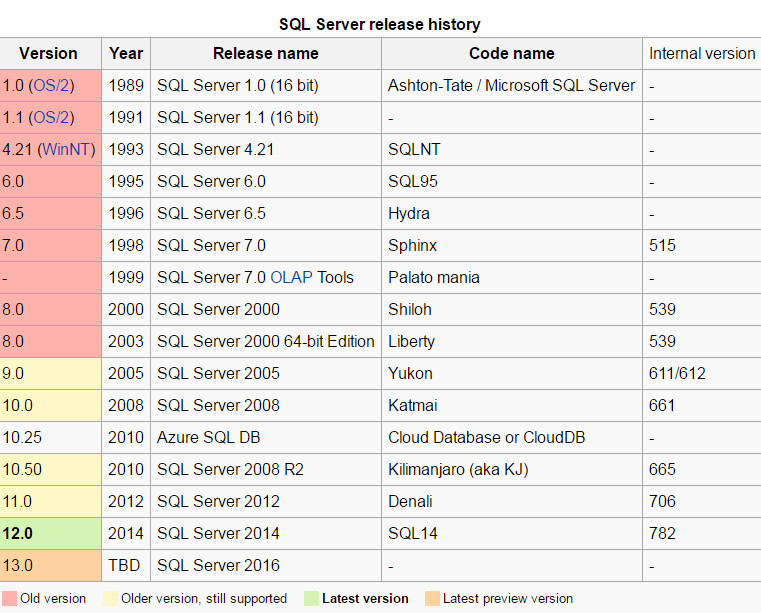
\includegraphics[width=1\linewidth]{image1.jpg}
\caption{History Microsoft SQL Server}
\label{fig:image1}
\end{figure}

\subsection{Architecture}
The protocol layer implements the external interface to SQL Server. All operations that can be invoked on SQL Server are communicated to it via a Microsoft-defined format, called  Tabular Data Stream (TDS). TDS is an application layer protocol, used to transfer data between a database server and a client. Initially designed and developed by Sybase Inc. for their Sybase SQL Server relational database engine in 1984, and later by Microsoft in Microsoft SQL Server, TDS packets can be encased in other physical transport dependent protocols, including TCP/IP, named pipes, and shared memory. Consequently, access to SQL Server is available over these protocols. In addition, the SQL Server API is also exposed over web services.

\subsection{Data Storage}
Data storage is a database, which is a collection of tables with typed columns. SQL Server supports different data types, including primary types such as Integer, Float,Decimal, Char (including character strings), Varchar (variable length character strings), binary (for unstructured blobs of data), Text (for textual data) among others. The rounding of floats to integers uses either Symmetric Arithmetic Rounding or Symmetric Round Down (Fix) depending on arguments:
\begin{verbatim}�SELECT Round(2.5, 0)
\end{verbatim}
gives 3.


Microsoft SQL Server also allows user-defined composite types (UDTs) to be defined and used. It also makes server statistics available as virtual tables and views (called Dynamic Management Views or DMVs). In addition to tables, a database can also contain other objects including views, stored procedures, indexes and constraints, along with a transaction log. A SQL Server database can contain a maximum of ${2}^{31}$ objects, and can span multiple OS-level files with a maximum file size of ${2}^{60}$ bytes (1 exabyte). The data in the database are stored in primary data files with an extension .mdf. Secondary data files, identified with a�.ndf extension, are used to allow the data of a single database to be spread across more than one file, and optionally across more than one file system. Log files are identified with the.ldf extension. 

Storage space allocated to a database is divided into sequentially numbered pages, each 8 KB in size. A page is the basic unit of I/O for SQL Server operations. A page is marked with a 96-byte header which stores metadata about the page including the page number, page type, free space on the page and the ID of the object that owns it. Page type defines the data contained in the page: data stored in the database, index, allocation map which holds information about how pages are allocated to tables and indexes, change map which holds information about the changes made to other pages since last backup or logging, or contain large data types such as image or text. While page is the basic unit of an I/O operation, space is actually managed in terms of an extent which consists of 8 pages. A database object can either span all 8 pages in an extent ("uniform extent") or share an extent with up to 7 more objects ("mixed extent"). A row in a database table cannot span more than one page, so is limited to 8 KB in size. However, if the data exceeds 8 KB and the row contains Varchar or Varbinary data, the data in those columns are moved to a new page (or possibly a sequence of pages, called an Allocation unit) and replaced with a pointer to the data. 

For physical storage of a table, its rows are divided into a series of partitions (numbered 1 to n). The partition size is user defined; by default all rows are in a single partition. A table is split into multiple partitions in order to spread a database over a computer cluster. Rows in each partition are stored in either B-tree or heap structure. If the table has an associated, clustered index to allow fast retrieval of rows, the rows are stored in-order according to their index values, with a B-tree providing the index. The data is in the leaf node of the leaves, and other nodes storing the index values for the leaf data reachable from the respective nodes. If the index is non-clustered, the rows are not sorted according to the index keys. An indexed view has the same storage structure as an indexed table. A table without a clustered index is stored in an unordered heap structure. However, the table may have non-clustered indices to allow fast retrieval of rows. In some situations the heap structure has performance advantages over the clustered structure. Both heaps and B-trees can span multiple allocation units. 

\subsection{Concurrency and Locking}
SQL Server allows multiple clients to use the same database concurrently. As such, it needs to control concurrent access to shared data, to ensure data integrity when multiple clients update the same data, or clients attempt to read data that is in the process of being changed by another client. SQL Server provides two modes of concurrency control: pessimistic concurrency and optimistic concurrency. 

When pessimistic concurrency control is being used, SQL Server controls concurrent access by using locks. Locks can be either shared or exclusive. Exclusive lock grants the user exclusive access to the data no other user can access the data as long as the lock is held. 

Shared locks are used when some data is being read multiple users can read from data locked with a shared lock, but not acquire an exclusive lock. The latter would have to wait for all shared locks to be released. Locks can be applied on different levels of granularity on entire tables, pages, or even on a per-row basis on tables. For indexes, it can either be on the entire index or on index leaves. The level of granularity to be used is defined on a per-database basis by the database administrator. While a fine grained locking system allows more users to use the table or index simultaneously, it requires more resources. So it does not automatically turn into higher performing solution. 

SQL Server also includes two more lightweigh �mutual exclusion�solutions latches and spinlocks which are less robust than locks but are less resource intensive. SQL Server uses them for DMVs and other resources that are usually not busy. SQL Server also monitors all worker threads that acquire locks to ensure that they do not end up in deadlocks in case they do, SQL Server takes remedial measures, which in many cases is to kill one of the threads entangled in a deadlock and rollback the transaction it started. To implement locking, SQL Server contains the Lock Manager. The Lock Manager maintains an in-memory table that manages the database objects and locks, if any, on them along with other metadata about the lock. Access to any shared object is mediated by the lock manager, which either grants access to the resource or blocks it.

SQL Server also provides the optimistic concurrency control mechanism, which is similar to the multi version concurrency control used in other databases. The mechanism allows a new version of a row to be created whenever the row is updated, as opposed to overwriting the row, i.e., a row is additionally identified by the ID of the transaction that created the version of the row. Both the old as well as the new versions of the row are stored and maintained, though the old versions are moved out of the database into a system database identified as Tempdb. When a row is in the process of being updated, any other requests are not blocked (unlike locking) but are executed on the older version of the row. If the other request is an update statement, it will result in two different versions of the rows both of them will be stored by the database, identified by their respective transaction IDs. 
\section{MySql}
MySQL is an open-source relational database management system (RDBMS);�in July 2013, it was the world's second most[a] widely used RDBMS, and the most widely used open-source�client server mode  RDBMS. It is named after co-founder Michael Widenius's daughter, My. The SQL abbreviation stands for Structured Query Language. The MySQL development project has made its source code available under the terms of the GNU General Public License, as well as under a variety of proprietary agreements. MySQL was owned and sponsored by a single�for-profit firm, the Swedish company MySQL AB, now owned by�.Oracle Corporation. For proprietary use, several paid editions are available, and offer additional functionality.

MySQL is a popular choice of database for use in web applications, and is a central component of the widely used LAMP open-source web application software stack (and other "AMP" stacks). LAMP is an acronym for "Linux, Apache, MySQL, Perl/PHP/Python". Free-software open-source projects that require a full-featured database management system often use MySQL. Applications that use the MySQL database include:�
\begin{itemize}
\item TYPO3
\item MODx
\item Joomla
\item WordPress
\item phpBB
\item MyBB
\item Drupal�
\item andother software
\end{itemize}

 MySQL is also used in many high-profile, large-scale websites, including Google (though not for searches), Facebook, Twitter, Flickr, and YouTube. 

On all platforms except Windows, MySQL ships with no GUI tools to administer MySQL databases or manage data contained within the databases. Users may use the included command line tools, or install MySQL Workbench via a separate download. Many third party GUI tools are also available.
\subsection{History}
MySQL was created by a Swedish company, MySQL AB, founded by David Axmark, Allan Larsson and Michael "Monty" Widenius. The first version of MySQL appeared on 23 May 1995. It was initially created for personal usage from mSQL based on the low-level language ISAM, which the creators considered too slow and inflexible. They created a new SQL interface, while keeping the same AP  as mSQL. By keeping the API consistent with the mSQL system, many developers were able to use MySQL instead of the (proprietarily licensed) mSQL antecedent
\begin{figure}[!th]
\centering
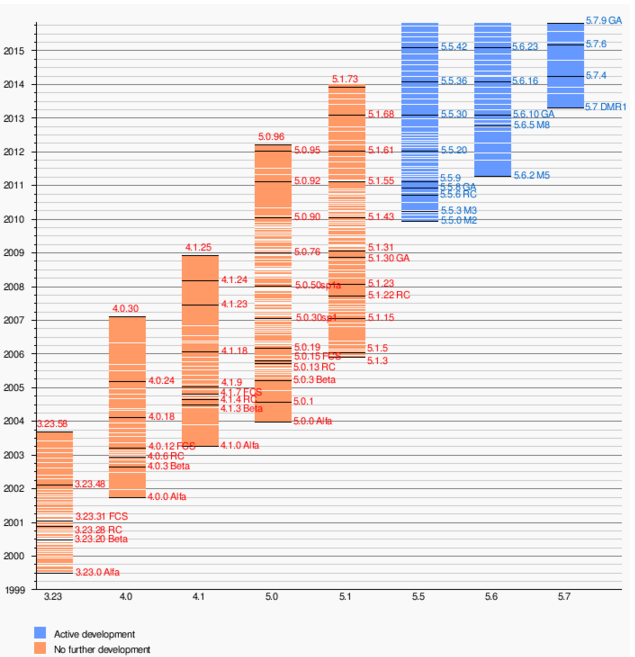
\includegraphics[width=1\linewidth]{image2}
\caption{Versions of MySQL}
\label{fig:image2}
\end{figure}


\subsection{Features}
MySQL is offered under two different editions: the open source MySQL Community Server and the proprietary Enterprise Server. MySQL Enterprise Server is differentiated by a series of proprietary extensions which install as server plugins, but otherwise shares the version numbering system and is built from the same code base.

Major features as available in MySQL 5.6:
\begin{itemize}
\item
A broad subset of ANSI SQL 99, as well as extensions
\item Cross-platform support
\item Stored procedures, using a procedural language that closely adheres to SQL/PSM
\item Triggers
\item Cursors
\item Updatable views
\item Online DD  when using the InnoDB Storage Engine.
\item Information schema
\item Performance Schema that collects and aggregates statistics about server execution and query performance for monitoring purposes.
\item A set of SQL Mode options to control runtime behavior, including a strict mode to better adhere to SQL standards.
\item X/Open XA distributed transaction processing�(DTP) support;two phase commit as part of this, using the default InnoDB storage engine
\item Transactions with savepoints when using the default InnoDB Storage Engine. The NDB Cluster Storage Engine also supports transactions.
\item ACID compliance when using InnoDB and NDB Cluster Storage Engines
\item SSL support
\item Query caching
\item Sub-SELECTs�(i.e. nested SELECTs)
\item Built-in Replication support (i.e. Master-Master Replication and Master-Slave Replication) with one master per slave, many slaves per master. Multi-master replication is provided in MySQL Cluster, and multi-master support can be added to unclustered configurations using Galera Cluster.
\item Full-text indexing and searching.
\item Embedded database library
\item Unicode support
\item Partitioned tables with pruning of partitions in optimizer
\item Shared-nothing clustering through MySQL Cluster
\item Multiple storage engines, allowing one to choose the one that is most effective for each table in the application.[d]
\item Native storage engines InnoDB, MyISAM, Merge, Memory (heap), Federated, Archive, CSV, Blackhole, NDB Cluster.
\item Commit grouping, gathering multiple transactions from multiple connections together to increase the number of commits per second.
\end{itemize}

The developers release minor updates of the MySQL Server approximately every two months. The sources can be obtained from MySQL's website or from MySQL's GitHub repository, both under the GPL license.
\subsection{Deployment}
MySQL can be built and installed manually from source code, but it is more commonly installed from a binary package unless special customizations are required. On most Linux distributions, the package management system can download and install MySQL with minimal effort, though further configuration is often required to adjust security and optimization settings.

Though MySQL began as a low-end alternative to more powerful proprietary databases, it has gradually evolved to support higher-scale needs as well. It is still most commonly used in small to medium scale single-server deployments, either as a component in a LAMP-based web application or as a standalone database server. Much of MySQL's appeal originates in its relative simplicity and ease of use, which is enabled by an ecosystem of open source tools such as phpMyAdmin. In the medium range, MySQL can be scaled by deploying it on more powerful hardware, such as a multi-processor server with gigabytes of memory.

There are however limits to how far performance can scale on a single server ('scaling up'), so on larger scales, multi-server MySQL ('scaling out') deployments are required to provide improved performance and reliability. A typical high-end configuration can include a powerful master database which handles data write operations and is replicate to multiple slaves that handle all read operations. The master server continually pushes binlog events to connected slaves so in the event of failure a slave can be promoted to become the new master, minimizing downtime. Further improvements in performance can be achieved by caching the results from database queries in memory using memcached, or breaking down a database into smaller chunks called shards which can be spread across a number of distributed server clusters.
\subsection{High availability}
Ensuring high availability requires a certain amount of redundancy in the system. For database systems, the redundancy traditionally takes the form of having a primary server acting as a master, and using replication to keep secondaries available to take over in case the primary fails. This means that the "server" that the application connects to is in reality a collection of servers, not a single server. In a similar manner, if the application is using a shared database, it is in reality working with a collection of servers, not a single server. In this case, a collection of servers is usually referred to as a farm.

One of the projects aiming to provide high availability for MySQL is MySQL Fabric, an integrated system for managing a collection of MySQL servers, and a framework on top of which high availability and database sharding is built. MySQL Fabric is open-source and is intended to be extensible, easy to use, and to support procedure execution even in the presence of failure, providing an execution model usually called resilient execution.�MySQL client libraries are extended so they are hiding the complexities of handling failover in the event of a server failure, as well as correctly dispatching transactions to the shards. As of September 2013, there is support for Fabric-aware versions of Connector/J, Connector/PHP, Connector/Python, as well as some rudimentary support for Hibernate and Doctrine. As of May 2014, MySQL Fabric is in the general availability stage of development.



\end{document}


